\chapter{Quadrifilare Helixantenne (QHA)}
\label{chap:qfh}
Die Quadrifilare Helixantenne ist eine Abwandlung der monofilaren Helixantenne und unterscheidet sich von dieser in mehreren wichtigen Punkten.

Zum einen ist sie um einiges kleiner als die monofilare Helix. Zum anderen wird sie als omnidirektionale Antenne für Satellitenkommunikation verwendet, da sie, wie die monofilare Helix, zirkular polarisiert ist. Allerdings zeigt sie entlang des Horizonts sowie direkt nach oben einen besseren Antennengewinn als in andere Richtungen.

\section{Funktionsweise}
Die QHA ist eine symmetrische Antenne, was bedeutet, dass sie mithilfe eines Baluns auf ein unsymmetrisches Koaxialkabel angepasst werden muss. Mehr dazu in Kapitel QUERVERWEIS.

Die QFH besteht aus einer größeren Schleife, welche unterhalb der gewollten Frequenz resonant ist, und einer kleineren Schleife, welche oberhalb der gewollten Frequenz resonant ist. Die größere Schleife bildet die kapazitive Komponente und die kleinere Schleife die induktive Komponente. Dadurch entsteht eine Phasenverschiebung von (ideal) 90° über die bifilaren Elemente. Werden die Streifen richtig dimensioniert, so ergibt sich eine gute zirkulare Polarisation, weichen sie ab so ergibt sich eine elliptische Polarisation.

\section{Design}
Das Design der QHA muss einigen Anforderungen entsprechen. Neben den Anforderungen die eigentliche Funktion zu erfüllen, scilicet für eine Frequenz von 433 Megahertz ein möglichst quasi-isotropes Abstrahlverhalten nach oben aufzuweisen und auf 50 Ohm angepasst zu sein, den Anforderungen durch die Natur gerecht zu werden. Dabei wird ein besonderes Augenmerk auf die UV-Resistenz und den Korrosionsschutz gelegt. 

Um Richtwerte für die Dimensionen einer QHA im 70cm-Band zu erhalten, wurde das Online-Tool unter \url{https://jcoppens.com/ant/qfh/calc.en.php} zur Dimensionierung von Antennen eingesetzt. Es ergeben sich dadurch folgende Werte:

\begin{center}
\begin{tabular}{|c|c|c|}
	\hline
	\textbf{Parameter} & \textbf{kleine Schleife} & \textbf{große Schleife} \\
	\hline
	\textbf{Durchmesser} & 96.1 Millimeter & 101.1 Millimeter \\
	\hline
	\textbf{Höhe} & 218.4 Millimeter & 229.9 Millimeter \\
	\hline
\end{tabular}
\end{center}

Mithilfe der Werte wurde folgendes 3D-Model der Antenne zur Simulation entworfen. Es gilt dabei zu erwähnen, dass, angetrieben von wissenschaftlicher Neugier, die QHA entgegen der typischen Konstruktion mit Kupferrohren aus Aluminiumstreifen simuliert und gefertigt wird. 

BILD - RENDER

Die Simulationsergebnisse der Antenne zeigen, dass sie bei einer Frequenz von 465 Megahertz die beste Performanz besitzt in Bezug auf die Anpassung besitzt. Bei dieser Frequenz erreicht sie eine Rückflussdämpfung von -16 Dezibel, was zwar nicht ideal, jedoch akzeptabel ist.

\begin{figure} [H]
	\centering
	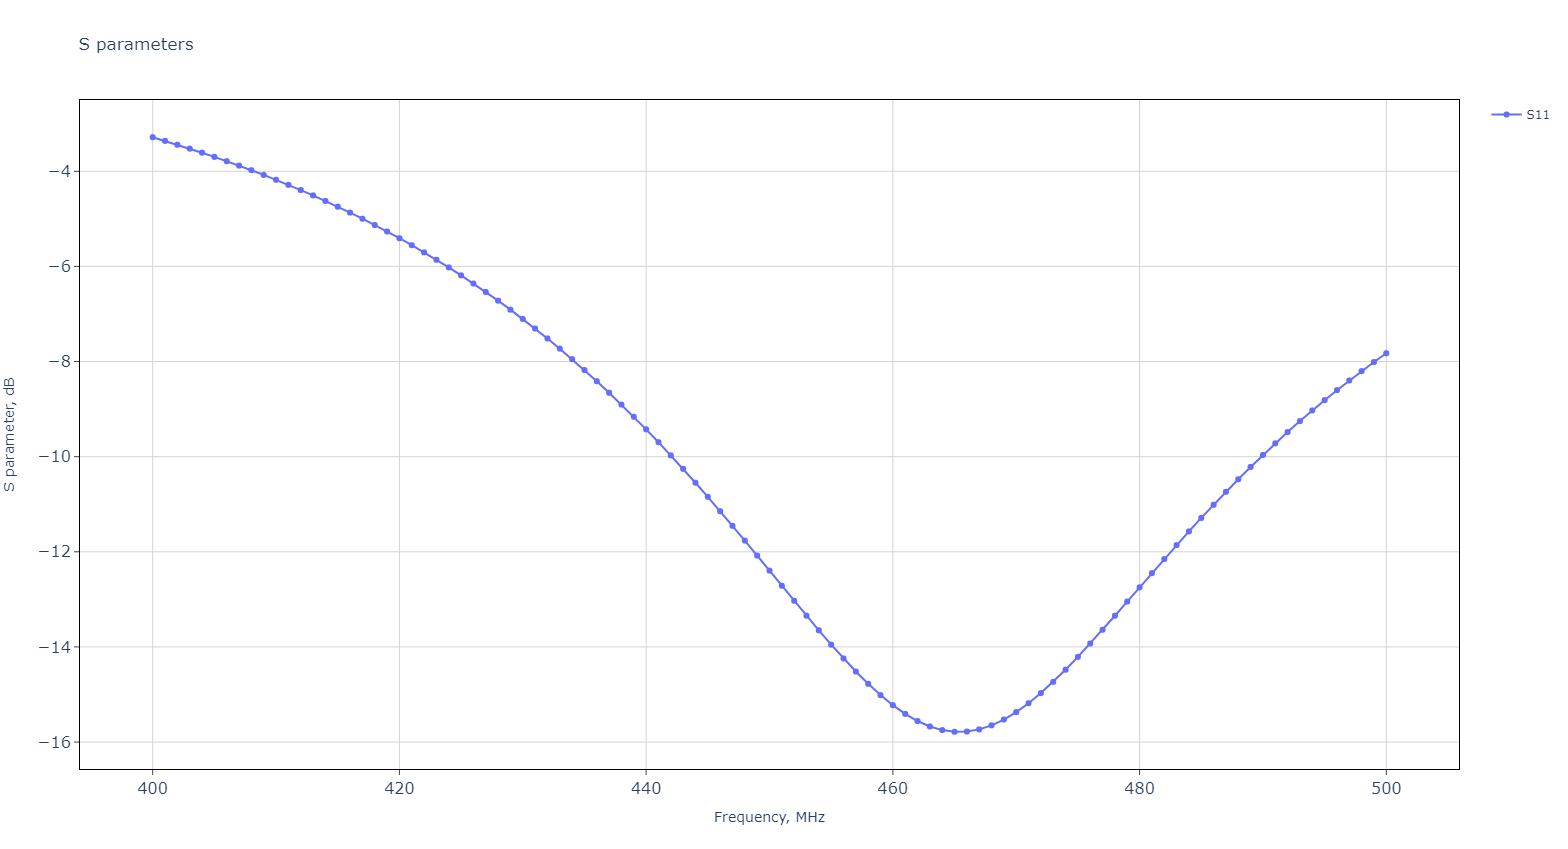
\includegraphics[width=\linewidth]{../ref/qfh_old_s11.png}
	\caption{S11-Parameter der ersten QHA}
	\label{fig:s11_old_qha}
\end{figure}

Das Abstrahlverhalten bei 465 Megahertz entspricht der Theorie und 

\begin{figure} [H]
	\centering
	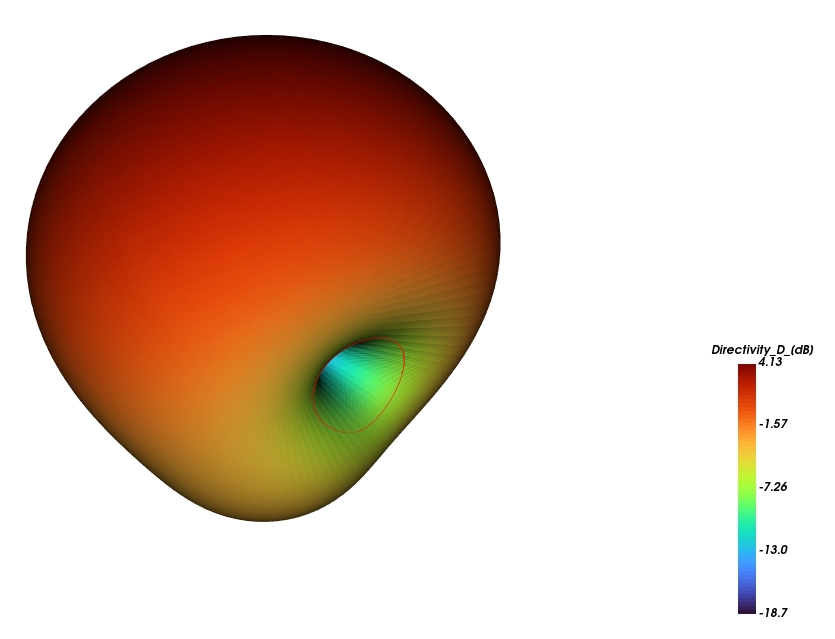
\includegraphics[width=\linewidth]{../ref/radiation_pattern_old_qfh.png}
	\caption{S11-Parameter der ersten QHA}
	\label{fig:rp_old_qha}
\end{figure}

\section{Realisierung}
Metallstreifen, metallrundlinge, Biegelehre, Balun?

BILD DER QFH

\section{Messungen}

